\section{Pengantar}
\begin{frame}{Pengantar}
\begin{figure}
	\centering
	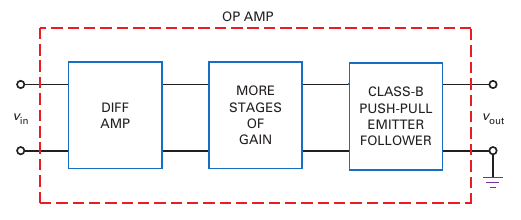
\includegraphics[width=0.7\linewidth]{gambar/fig-16.01}
	\caption{Blok diagram sebuah op amp}
	\label{fig-16.01}
\end{figure}
\end{frame}

\begin{frame}{Pengantar}
	\begin{figure}
		\centering
		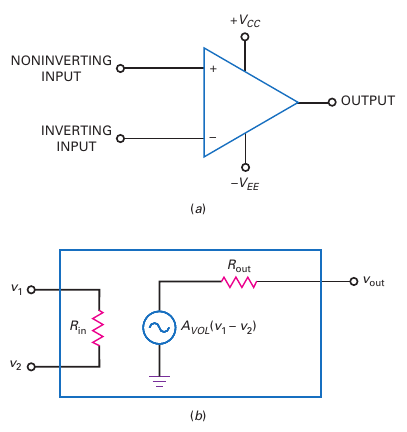
\includegraphics[width=0.4\linewidth]{gambar/fig-16.02}
		\caption{(a) Simbol dari op amp dan (b) rangkaian ekivalen dari op amp}
		\label{fig-16.02}
	\end{figure}
\end{frame}

\begin{frame}{Pengantar}
	\begin{figure}
		\centering
		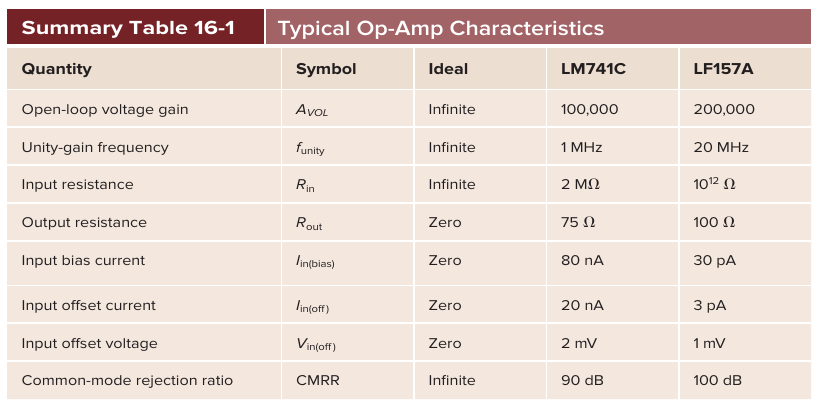
\includegraphics[width=0.8\linewidth]{gambar/tab-16.01}
		\caption{Perbandingan karakteristik op amp ideal dan op amp standar}
		\label{tab-16.01}
	\end{figure}
\end{frame}